To manage our software we are using \textit{Rust},
as the main language of development, due to its high expressibility and low level management.
We utilise methods such as Test-Driven-Development with the help of \texttt{Proptest}
for property testing and kanban boards to accurately track our progress as seen
in figure \ref{fig:soft:ecs-workflow}. Lastly we are making use of 
\textit{Bevy} which is a game engine that uses the Entity-Component-System
architecture to render interactions between entities as seen in \ref{fig:soft:ecs-workflow} \cite{bevyengine}.


\begin{figure}[h!]
    \centering
    \subfloat[ECS workflow visualisation. Entities which exist in a world state are equipped with components.
    Systems query entities with specific components and modify the world state.]{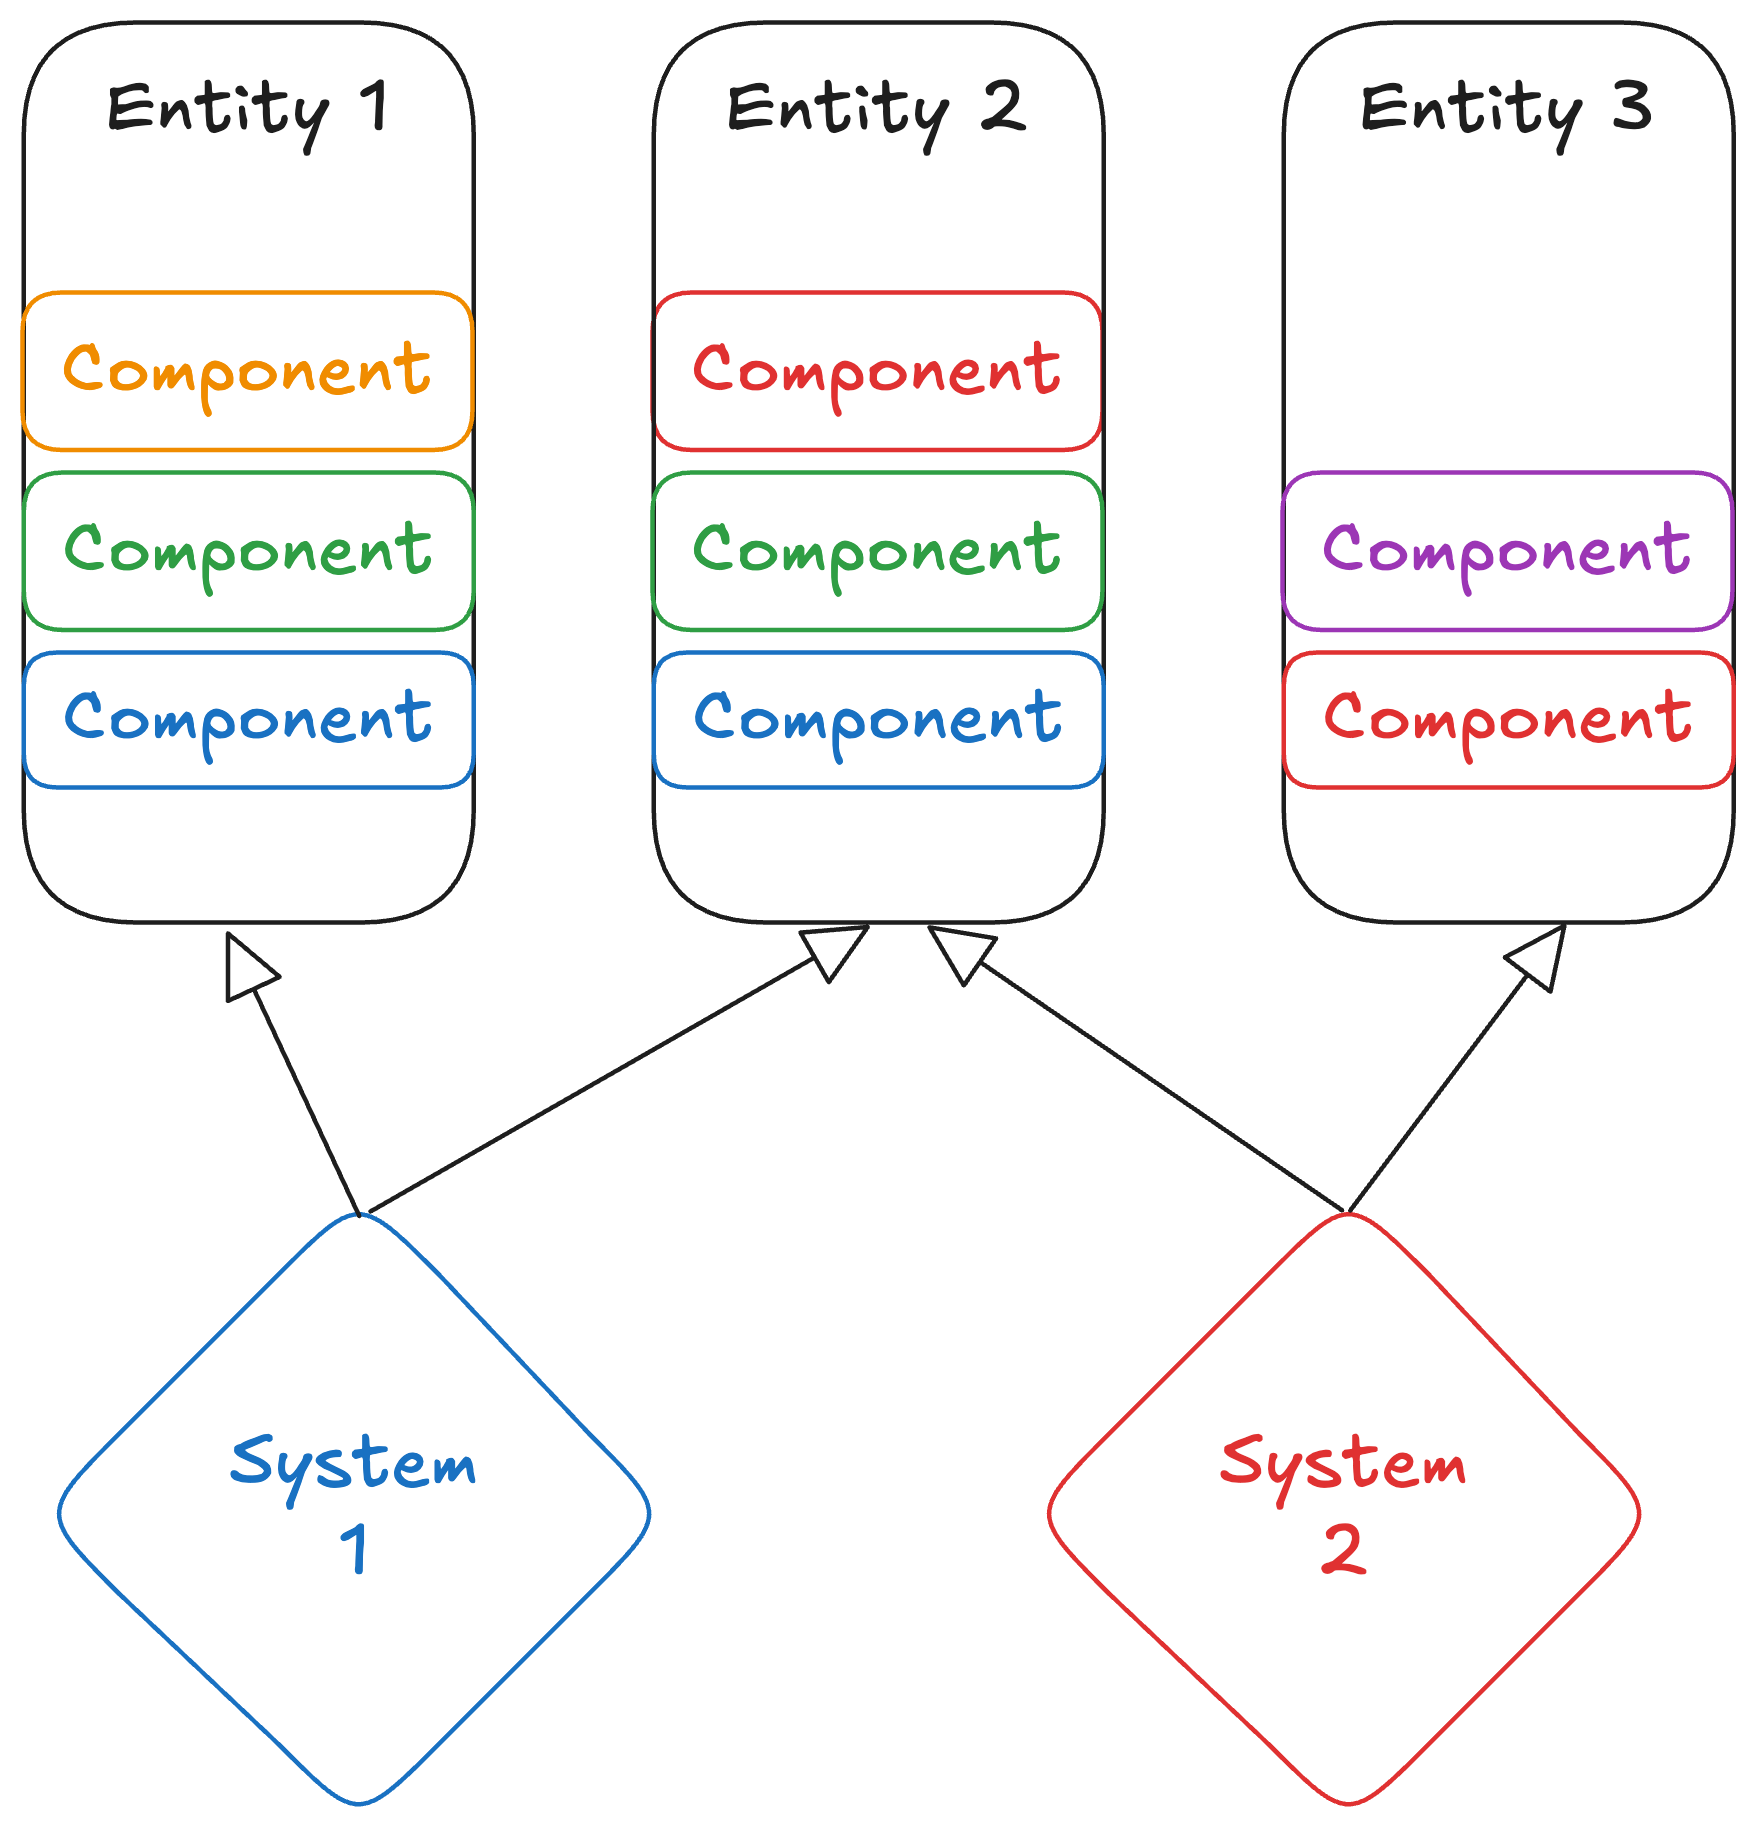
\includegraphics[width=0.4\linewidth]{assets/ECS-visualisatoin.png}}
    \hfill
    \subfloat[Kanban board]{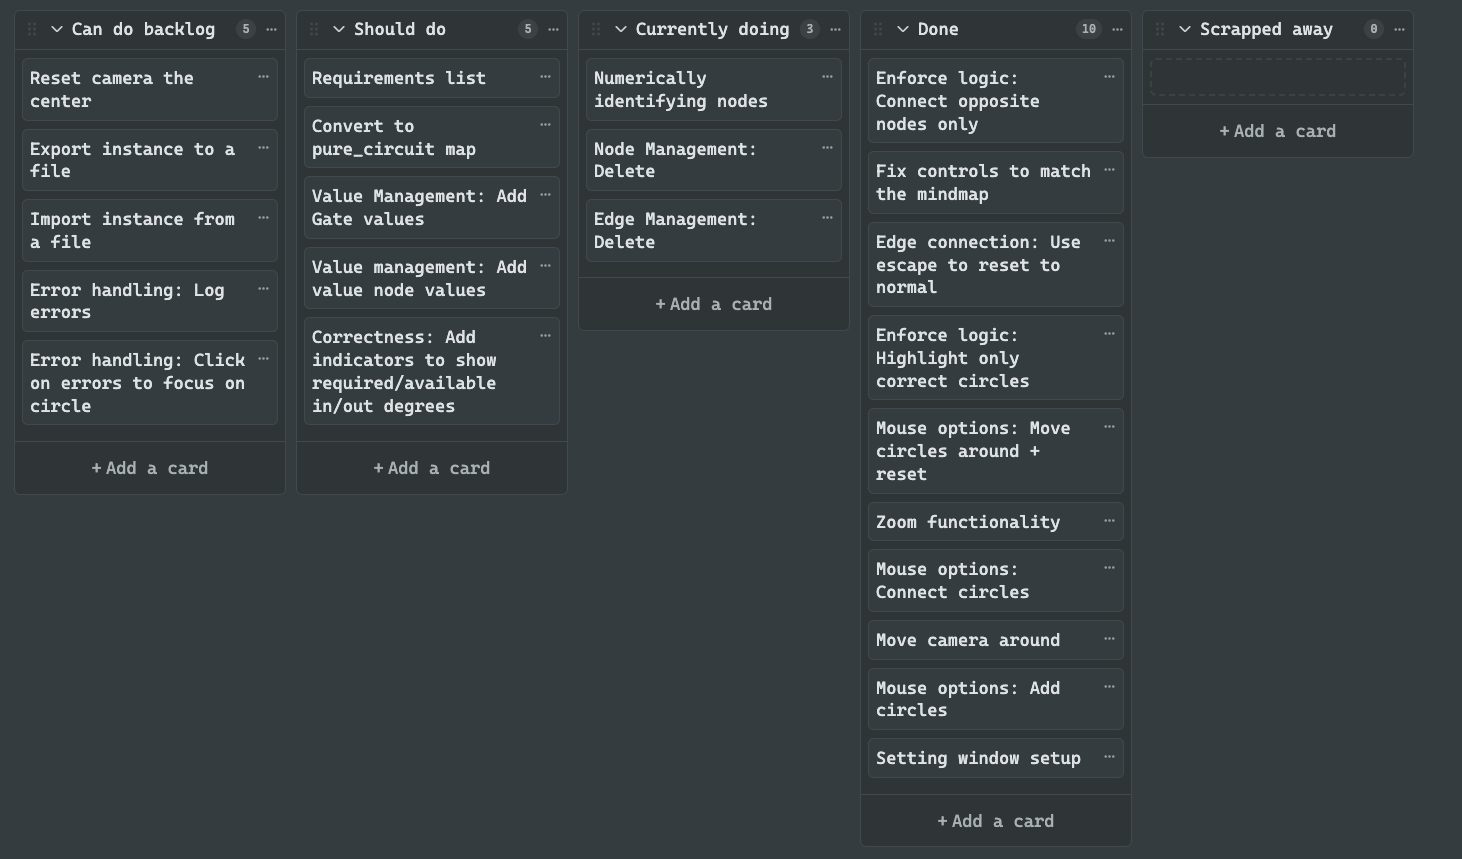
\includegraphics[width=0.4\textwidth]{assets/kanban-board.png}}
    \caption{Software management}
    \label{fig:soft:ecs-workflow}
\end{figure}

With regards to the our research management, we revolved our work around obsidian.
As we can observe in the figure \ref{fig:theory:obsidian-usages}, 
\texttt{Obsidian} beyond its traditional usage of note taking, entails several handy tools such as note organisation and mind-mapping.



\begin{figure}[h!]
    \centering
    \subfloat[Obsidian Graph]{
        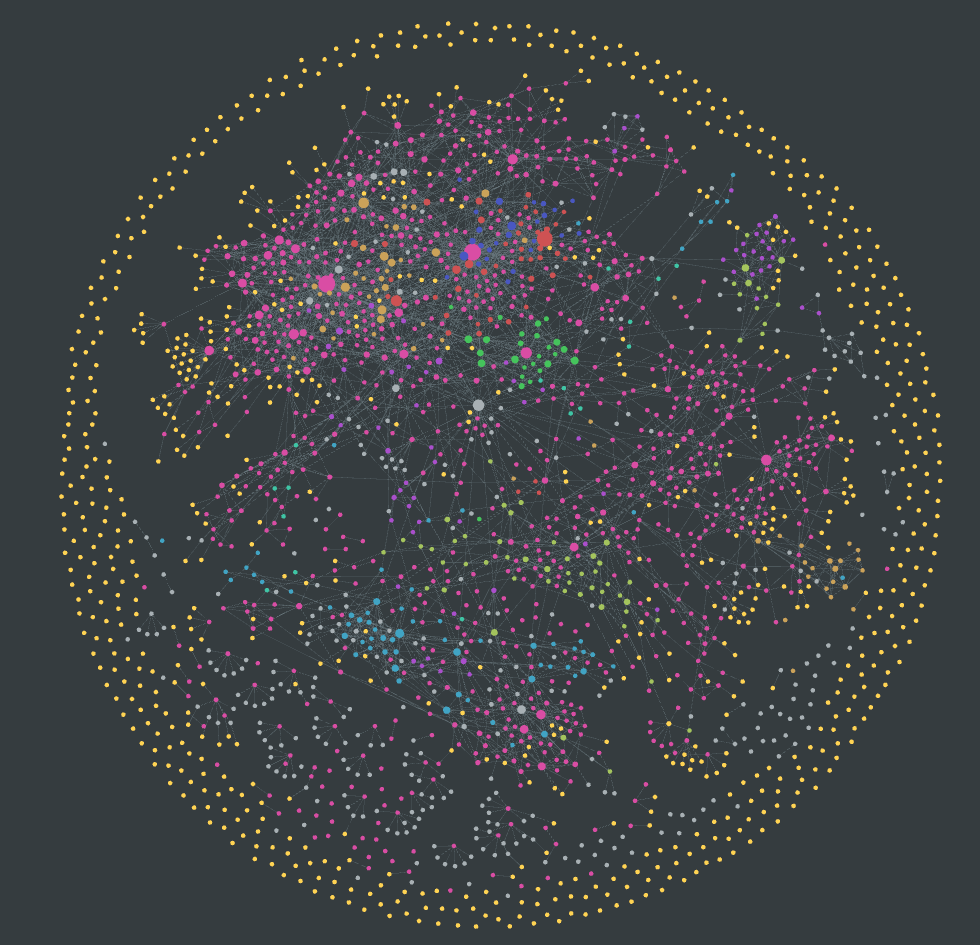
\includegraphics[width=0.3\linewidth]{assets/obsidian_graph.png}
        \label{fig:theory:obsidian-graph}
    }
    \subfloat[Obsidian Canvas]{
        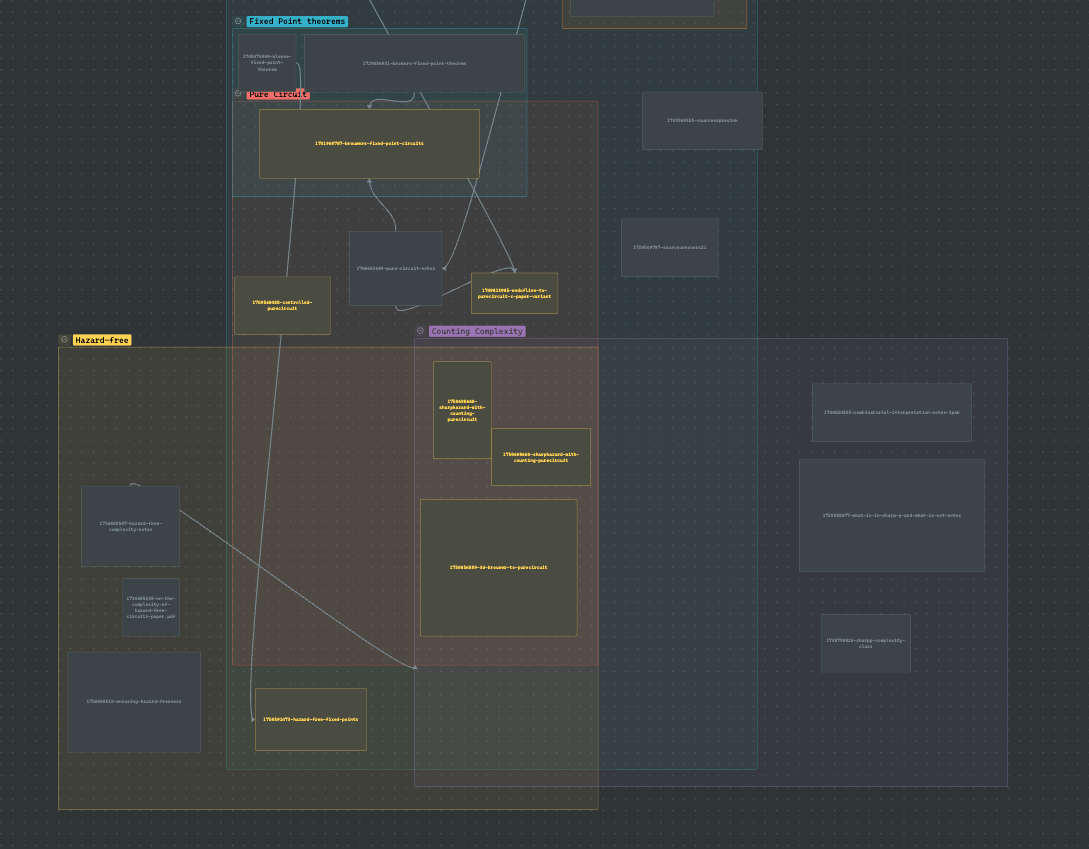
\includegraphics[width=0.3\linewidth]{assets/obsidian-canvas.png}
        \label{fig:theory:obsidian-canvas}
    }
    \subfloat[Obsidian mindmap]{
        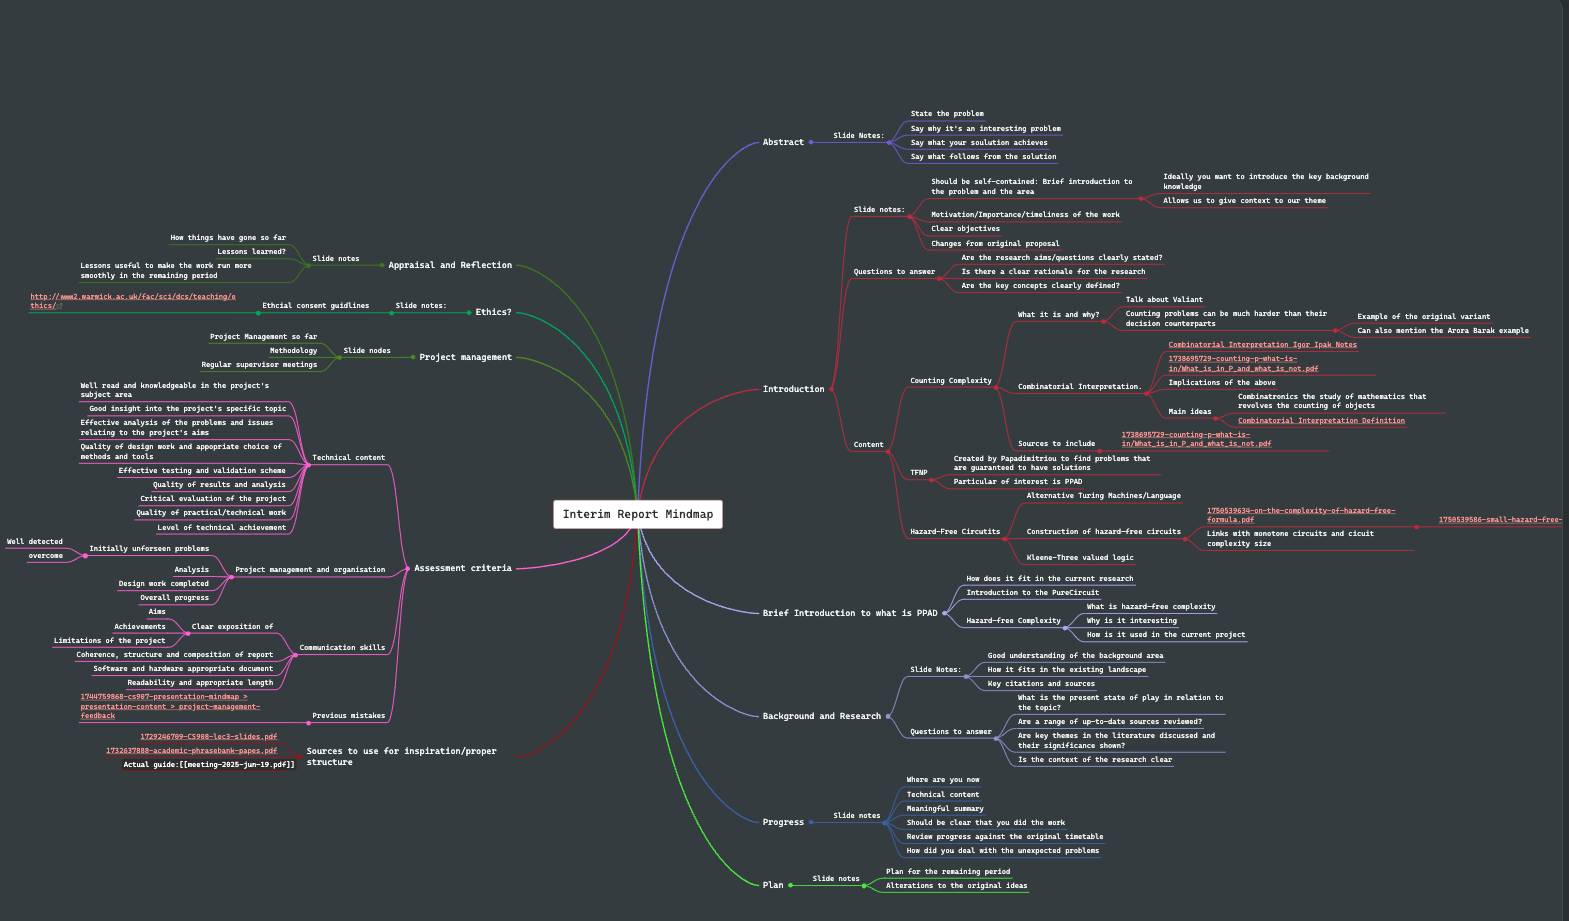
\includegraphics[width=0.3\linewidth]{assets/obsidian_mindmap.png}
        \label{fig:theory:obsidian-mindmap}
    }
    \caption{Usages of Obsidian}
    \label{fig:theory:obsidian-usages}
\end{figure}



\subsection{Risk Management}

Due to the limited prior research on the counting complexity of $\textsc{\#TFNP} -1$,
this project involved significant risks.
Our justification for the proposed milestones was largely informed by existing knowledge regarding the complexity of circuit constructions.
However, it remained entirely possible that our proposed reductions could prove to be infeasible.
Furthermore, working with Kleene logic introduced additional complexity, and it maybe the reason why 
establishing fully parsimonious reductions between the target problems may not be achievable.
This is also the reason why we diverted our attention to bounded parsimonious reductions instead.
A detailed overview of the associated risks and our proposed mitigation strategies is provided in the table \ref{tab:management:risk-management}.


\begin{xltabular}{0.95\linewidth}{|Z{1.2cm}|Z{1.75cm}|Y|Y|Z{1.2cm}|}
        \hline
        \textbf{Severity} & \textbf{Probability} & \textbf{Description} & \textbf{Mitigation} & \textbf{Address} \\
        \hhline{|=|=|=|=|=|}
        High   & Medium & Software may not be feasible within the remaining time frame. & We focus on the validation and creation of instances.
        The current project is primarly research-based, and therefore we are mainly prioritising the theory development aspect of the project. & Not yet      \\ \hline
        Low    & Medium & Software not identifying a correct solution & Usage of TDD techniques and property testing to ensure correctness.  Comparison with hand-made instances. & Not yet      \\ \hline
        Medium & Low    & Difficulty of showing the parsmonious reduction between  \textsc{PureCircuit} and  \textsc{nD-StrongSperner} & Consult with the researchers that actively work on these problems. Lower the requirements
               to polynomially bounded reductions instead. &  Not yet \\ \hline
        High   & High   & Inability to make significantt progress on the \textsc{SourceOrExcess} problems or the generalised statement &
        Establish reductions from other problems in order to demonstrate \textsc{\#P} hardness by starting from $\textsc{nD-StrongSperner}$& Not yet \\ \hline
        High   & High   & Incorrect proofs or reductions. &
        Analyse the problem under different constraints.
            Apply the duck method, where attempt to explain the solution to a person which not necessarily an expert. Validate proof with supervisor or
               use the tool to investigate sample cases. & On-going  \\ \hline
        High   & Medium & Develop combinatorial friendly variants of \textsc{PureCircuit} & Apply robustness on the gate set of \textsc{PureCircuit}. Develop new gates or variants are easier to work with or work
        on a subset of solutions as explained in \ref{par:pure-circ-def} & $\checkmark$  \\ \hline
        \caption{Risk management table.} \label{tab:management:risk-management}
\end{xltabular}

%
% From our table, it is worth expanding on some of the points. The best method
% we found when tackling this problem is when we try to uncover reductions between other
% \textsc{PPAD} problems or when trying to incorporate gadgets from Kleene theory. We hope
% that by experimenting enough we will be able to get close to resolve our conjectures.
%
